\appendix
\chapter{Applied in CPlan}
\section{K-Means Clustering Options}
To apply centroid based clustering to a street network a specialized gui dialog was created where all parameters can be set. As you can see in figure \ref{fig:applied_k-means_GUI}.
\begin{itemize}
    \item If 'Show Visualisation' is activated the clustering process will be visualized.
    \item The counter 'Number of Tries' represents the count how often the clustering algorithm will be executed to extract the best result.
    \item 'Iterations per Try' describe how many iterations are maximal made per try. 
    \item If 'Shortest Path' is selected a shortest path algorithm will be applied after the centroid were set.
\end{itemize}
\begin{figure}[ht]
    \centering
    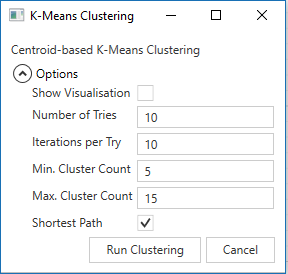
\includegraphics[width=0.47\linewidth]{k-means_clustering_applied.png}
    \caption{This gui dialog represents the parameters which could be applied to the K-Mean clustering algorithm.}
    \label{fig:applied_k-means_GUI}
\end{figure}

\section{Hierarchical Clustering Options}
A specialized gui was created to set parameters for the hierarchical clustering analysis. The reduction formula can be selected at the top \ref{fig:applied_HC_clustering_GUI}.
\begin{itemize}
    \item If the option 'Show Slider Dialog' is selected the cluster count can be changed in an additional dialog \ref{fig:applied_HC_clustering_slider_GUI}.
    \item The field 'Number of Clusters' represents the number of clusters which will be generated.
    \item If 'Modify Output' is selected always the biggest cluster will be split instead as the hierarchy was created.
\end{itemize}

\begin{figure}[ht]
    \centering
    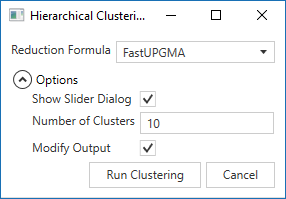
\includegraphics[width=0.47\linewidth]{HC_clustering_applied.png}
    \caption{This gui dialog represents the parameters which could be applied to the hierarchical clustering algorithm.}
    \label{fig:applied_HC_clustering_GUI}
\end{figure}

\begin{figure}[ht]
    \centering
    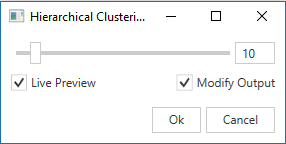
\includegraphics[width=0.47\linewidth]{HC_clustering_applied_slider.png}
    \caption{This gui dialog represents the optional 'Slide Dialog' which allows direct changes of the cluster count.}
    \label{fig:applied_HC_clustering_slider_GUI}
\end{figure}

\pagebreak
\section{Cluster Measurement Options}
To compare clusters the process was visualized for this thesis. A dialog allows to select two clusters and compare the measured results \ref{fig:applied_clustering_analysis_GUI}. The selected clusters are marked by colours in the main view \ref{fig:applied_clustering_analysis_visualized_GUI}.

\begin{figure}[ht]
    \centering
    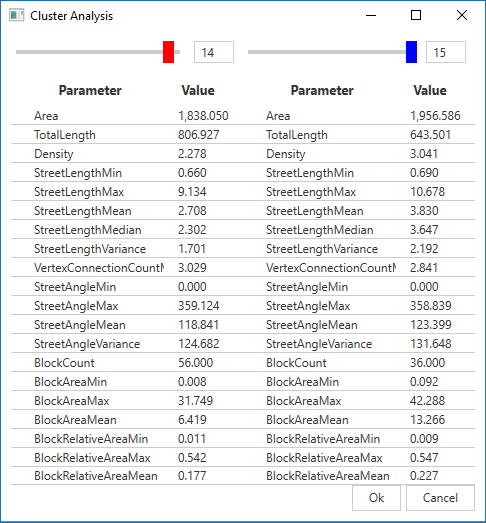
\includegraphics[width=0.8\linewidth]{cluster_applied_compare.png}
    \caption{This gui dialog allows to select two clusters and to compare the measured values.}
    \label{fig:applied_clustering_analysis_GUI}
\end{figure}

\begin{figure}[ht]
    \centering
    \begin{mdframed}[style=border]
        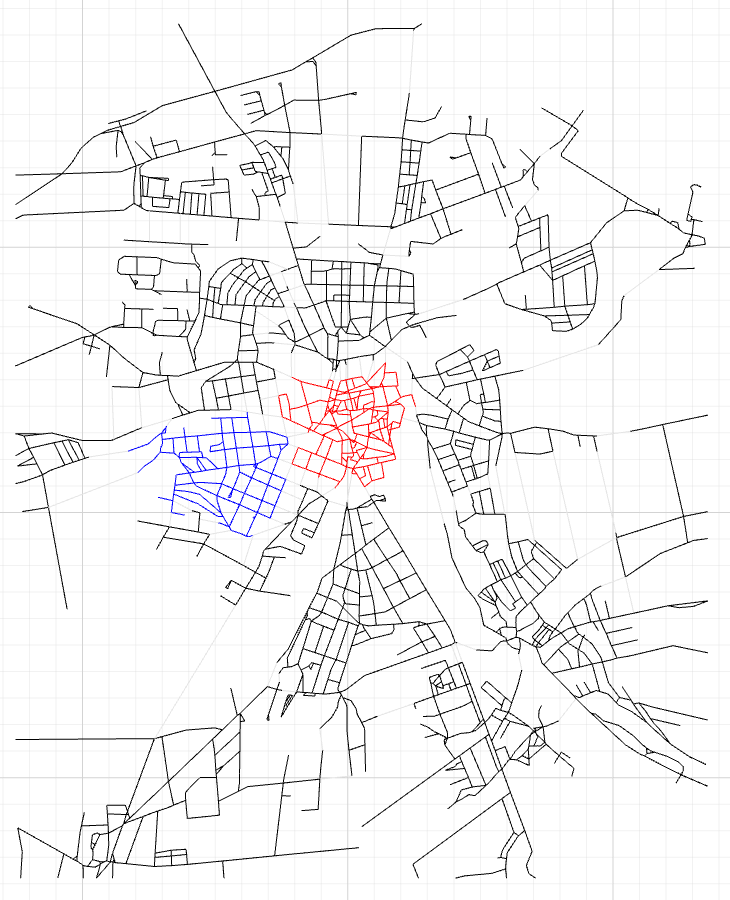
\includegraphics[width=\linewidth]{cluster_applied_compare_visualized.png}
    \end{mdframed}
    \caption{Main view with marked from the 'Cluster Analysis' dialog}
    \label{fig:applied_clustering_analysis_visualized_GUI}
\end{figure}

\FloatBarrier
\section{Measured Clusters}
\label{sec:measurements_full_table}
This table represent the full measured data with the cluster analysis method.

\begin{table}[h]
    \begin{center}
        \begin{tabular}{ |l|l|l|l|l| }
            \hline
            \textbf{Parmate}r &
            & \textbf{C1} \ref{sec:historyDistinct}
            & \textbf{C2} \ref{sec:businessDistinct}
            & \textbf{C3} \ref{sec:outskits}  \\ 
            \hline
            \multirow{4}{*}{Total} 
            & Area & 1838.05 & 1956.59 & 7802.74 \\
            & Length & 806.92 & 643.50 & 1069.81 \\
            & Density & 2.28 & 3.04 & 7.29 \\
            \hline
            \multirow{5}{*}{Street Length}
            & Min & 0.66 & 0.69 & 0.73 \\
            & Max & 9.13 & 10.68 & 38.00 \\
            & Mean & 2.72 & 3.85 & 4.82 \\
            & Median & 2.30 & 3.65 & 3.28 \\
            & Variance & 1.70 & 2.19 & 5.00 \\
            \hline
            \multirow{1}{*}{Vertex} 
            & Connections & 3.04 & 2.84 & 2.45 \\
            \hline
            \multirow{5}{*}{Street Angle} 
            & Min & 0.00 & 0.00 & 0.00 \\
            & Max & 151.80 & 358.84 & 359.80 \\
            & Mean & 119.03 & 123.75 & 137.18 \\
            & Variance & 124.68 & 131.65 & 129.47 \\
            \hline
            \multirow{5}{*}{Block} 
            & Count & 55 & 35 & 26 \\
            & Area Min & 0.01 & 0.09 & 0.00 \\
            & Area Max & 31.75 & 42.29 & 567.26 \\
            & Area Mean & 6.54 & 13.65 & 76.30 \\
            & A/Ac Min & 0.01 & 0.01 & 0.00 \\
            & A/Ac Max & 0.54 & 0.55 & 0.66 \\
            & A/Ac Mean & 0.18 & 0.23 & 0.18 \\
            \hline
            \multirow{5}{*}{Integration} 
            & Min & 0.46 & 0.48 & 0.60 \\
            & Max & 0.57 & 0.75 & 1.0 \\
            & Mean & 0.49 & 0.59 & 0.78 \\
            \hline
            \multirow{5}{*}{Choice}
            & Min & 0.00 & 0.00 & 0.00 \\
            & Max & 1.00 & 0.67 & 0.34 \\
            & Mean & 0.10 & 0.05 & 0.04 \\
            \hline
        \end{tabular}
        \caption{Measured results from Historic District (C1) \ref{sec:historyDistinct}, Business District (C2) \ref{sec:businessDistinct} and Outskirts Area (C3) \ref{sec:outskits}}
    \end{center}
\end{table}

\pagebreak
\section{Guideline Source Code}
This section provides a guideline through the important parts of the C\# source code, which was developed during this thesis. It's meant as an entry point which can be used to navigate more easily through the code, which implements the discussed concepts.
%TODO


\pagebreak
\section{CPlan Improvements}
This chapter was created to inform the reader about certain improvements and observations made in the application CPlan \ref{CPlan}.
\begin{itemize}
    \item Some calls to the methods IEnumerable.ToArray() and IEnumerable.ToList() were removed. This method creates a new array / list and stores every item of the IEnumerable in this new collection. As a result the application had an extremely large footprint. To further reduce this overhead some methods were changed to take IEnumerable parameters instead of arrays.
    \item Certain graph and geometry extension methods were fixed. It would be good practice to create unit tests for such methods.
    \item The vector represented by the class Matrix2d is clockwise despite the norm is counter clockwise.
    \item Line intersections of the class Geometry2D was not correct detected an therefore corrected.
\end{itemize}
